\documentclass{article}[12pt]
\renewcommand{\baselinestretch}{1.5}
\setlength{\parskip}{1em}

\usepackage[parfill]{parskip}
\usepackage[affil-it]{authblk}
\usepackage[space]{grffile}

\usepackage[a4paper]{geometry}
\usepackage[latin1]{inputenc}
\usepackage[english]{babel}

\geometry{verbose}
\usepackage{float}
\usepackage{graphicx}
\usepackage{setspace}
\usepackage{caption}

\usepackage{latexsym,textcomp,longtable,tabulary}
\usepackage{booktabs,array,multirow,braket}
\usepackage{amsfonts,amsmath,amssymb,mathbbol,calc,cancel}
\usepackage{subfigure,color,blindtext,enumitem,siunitx}
\usepackage[colorinlistoftodos]{todonotes}

\usepackage{mathtools}
\usepackage{url,hyperref,etoolbox}
\numberwithin{equation}{section}
\hypersetup{colorlinks=false,pdfborder={0 0 0}}

%+figure layout options
\restylefloat{figure}
\setlist{leftmargin=*,before=\setlength{\rightmargin}{\leftmargin}}
\graphicspath{{./figures/}{docs/figures/}}

\providecommand\citet{\cite}
\providecommand\citep{\cite}
\providecommand\citealt{\cite}

\makeatletter
\makeatother


\title{Inference of Bifurcations\\with Differentiable Continuation}
\author{
        Gregory Szep\\King's College London\\London, WC2R 2LS\\
        \texttt{gregory.szep@kcl.ac.uk}
    \And
        Attila Csik\'asz-Nagy\\King's College London\\London, WC2R 2LS\\
        \texttt{attila.csikasz-nagy@kcl.ac.uk}
    \And
        Neil Dalchau\\Microsoft Research Cambridge\\Cambridge, CB1 2FB\\
        \texttt{ndalchau@microsoft.com}
}

\begin{document}
\newcommand{\rates}{F_{\theta}}
\newcommand{\tangent}{T_{\theta}}
\newcommand{\steadystates}{\partial S_{\theta}}

\newcommand{\Det}{\left| \frac{\partial\rates}{\partial u} \right|}
\newcommand{\measure}{\Psi_{\theta}}

\newcommand{\predictions}{\mathcal{P}}
\newcommand{\targets}{\mathcal{D}}
\newcommand{\loss}{L}

\newcommand{\Reals}{\mathbb{R}}
\maketitle

\begin{abstract}
    In this work we propose a gradient-based semi-supervised approach for matching target bifurcations with parameterised differential equation models. The cost function contains a supervised error term that is minimal when predicted bifurcations match the targets and an unsupervised bifurcation measure which acts as a proxy for the probability of a bifurcation, yielding non-zero gradients in non-bifurcating parameter regimes. The calculation of gradients with respect to parameters shares the same computational complexity as deflated pseudo-arclength continuation used to calculate the bifurcation diagram. Our implementation leverages automatic differentiation methods in Julia and we demonstrate model synthesis with minimal models which explore the space of saddle-node and pitchfork diagrams and the genetic toggle switch from synthetic biology. Furthermore, the cost landscape allows us to  organise models in terms of topological and geometric equivalence.
\end{abstract}

\section{Introduction}

Backpropagation through differential equation solves has been a breakthrough over the past couple of years \cite{Chen2018NeuralEquations,Rackauckas2019DiffEqFlux.jl-AEquations} that enabled scalable parameter inference for differential equations. Determining what model parameters should be for a given set of observations, in the setting of biology and engineering, are known as inverse problems \cite{Abdulla2009InverseBiology}.

Optimisation targets, however, have mostly been expressed in the spatio-temporal domain. Acquisition of such data can be costly and can often contain over-constraining information generated by processing steps or the measurement device rather than the state variables that underpin the observed mechanism. In microscopy, for example, data is often reported in arbitrary fluoresce units allowing the observer to shift and scale data arbitrarily. Furthermore, such data may also not contain sufficient information about dynamical transients in order to identify kinetic parameters. The emerging picture suggests that identification of the qualitative behaviour -- the bifurcation diagram -- should precede any attempt at inferring kinetic parameters \cite{Stumpf2019ParameterBifurcations}. Techniques for back-propagating through implicit equation solvers have also been developed \cite{Look2020DifferentiableLayers,Bai2019DeepModels} although to the best of the authors' knowledge have not been applied to bifurcation diagrams at the time of writing this paper.

In this work we propose a gradient-based semi-supervised approach that focuses on fitting high-level qualitative constraints, defined by state space structures, rather than kinetics. Drawing inspiration from implicit solvers \cite{Look2020DifferentiableLayers,Bai2019DeepModels} to calculate gradients we find that their computation shares the same  complexity as the algorithm used to calculate the bifurcation diagram. We use a predictor-corrector method called deflated pseudo-arclength continuation \cite{Farrell2016TheDiagrams,Veltz2019PseudoArcLengthContinuation.jl}, originally developed for partial differential equations. In the case of partial differential equations the computational complexity of calculating a single bifurcation diagram is not bounded since superpositions of localised solutions may give rise to uncountably many branches \cite{Avitabile2010ToEquation}. The complexity of computing a single branch, however, is bounded by the complexities of the chosen eigenvalue solver and corrector, and further decreased by adaptive stepping procedures \cite{Aruliah2016AlgorithmContinuation}.

We find that the cost function landscape contains basins that not only allow us to synthesise models with a desired bifurcation structure but also allow us to organise models in terms of topological and geometric equivalence. We discuss the relevance of this in model selection. In summary, our paper has the following main contributions:

\begin{itemize}
    \item Defined a differentiable semi-supervised cost function for encouraging and placing co-dimension one bifurcations to user-specified target locations
    \item Implementation of method in Julia package \texttt{FluxContinuation.jl} leveraging automatic differentiation tooling in \texttt{Flux.jl}
    \item Leveraging the cost landscape for a novel way of organising differential equation models in terms of geometric and topological equivalence
\end{itemize}

\subsection{Related Works | \textit{in progress}}

\paragraph{Bifurcation control} and \textit{inverse} bifurcation analysis literature applies control theory to enable design and identification of dynamical systems with qualitative constraints. The first works involved the calculation of the minimal distances to bifurcation manifolds \cite{Iwasaki1997AnType,Lu2006InverseSystems,Dobson2004DistanceBifurcations}. Those optimisations did not involve closed form expressions and the challenge of finding the manifolds to being with was left to random sampling.

\paragraph{Matching vector fields} From a dynamical systems perspective a given bifurcation curve constrains a state-vector field geometry. A set of target bifurcations may also be represented as a vector field flow and thus inferring bifurcations becomes a problem in matching flows in vector sub-spaces. Note that this would involve matching direction but not the magnitude of the flow.

\begin{itemize}
    \item smooth and match estimator methods \cite{Ranciati2017BayesianParameters}
    \item robots learning limit cycles \cite{Khadivar2021LearningBifurcations}
\end{itemize}

\paragraph{Non-differentiable methods} 
A large body of work is dedicated to finding conditions for fold-bifurcations, multistability and other

\begin{itemize}
    \item bifurcation inference using Mixed Integer Nonlinear Programming \cite{Otero-Muras2018Optimization-basedModels}
    \item Random sampling and genetic algorithms \cite{Chickarmane2005BifurcationTool,Conrad2006BifurcationClock}
\end{itemize}

\subsection{Preliminaries}
Suppose we parameterise a set of differential equations for states $u\in\Reals^N$ with a function $\rates$ in an unknown parameter space $\theta\in\Reals^M$. We would like these differential equations to obey a set of target bifurcations $\targets:=\{p_1\dots p_K\}$ along a known bifurcation parameter $p\in\Reals$. Let the differential equations be defined as
\begin{align}
	\partial_t u=\rates(z)
	\qquad\mathrm{where}\quad z:=(u,p)\quad
	\rates : \Reals^{N+1}\rightarrow\Reals^N
	\label{eq:model}
\end{align}
For a given set of parameters $\theta$ one could compute the set of predicted bifurcations $\predictions(\theta)$ using parameter continuation methods \cite{Veltz2019PseudoArcLengthContinuation.jl,Farrell2016TheDiagrams}. Our goal is to find optimal parameters $\theta^*$ that match predictions $\predictions(\theta^*)$ to specified targets $\targets$. We must design a suitable cost function $\loss$ so that
\begin{align}
    \theta^* := \mathrm{argmin}_{\theta} \loss(\theta|\targets)
    \label{eq:optimal-theta}
\end{align}
The optimal $\theta^*$ is not expected to always be unique, but is in general a manifold representing the space of qualitatively equivalent models. The cost function $\loss$ must have some distance measure between the two sets $\predictions(\theta)$ and $\targets$ with a bias that encourages equivalent cardinality $|\predictions(\theta)|=|\targets|$. This is especially important in the case where there are no predictions $|\predictions(\theta)|=0$.

For clarity, we guide the reader through the methods with the following minimal models that explore the space of saddle-nodes $\rates(z) = p + \theta_{1}u+\theta_{2}u^3$ and pitchforks $\rates(z) = \theta_{1} + p u+\theta_{2}u^3$. These minimal models are shown with targets $\targets$ in Figure \ref{fig:saddle-node} and Figure \ref{fig:pitchfork} respectively. These figures show that the determinant $\Det=0$ at the bifurcations and that its directional derivative along the bifurcation curve $\frac{d}{ds}\Det$ is finite and non-zero, at least in the non-degenerate case. This gives us our first hint of what should be optimised to increase the number of predictions $|\predictions(\theta)|$.

\begin{figure}
\centering
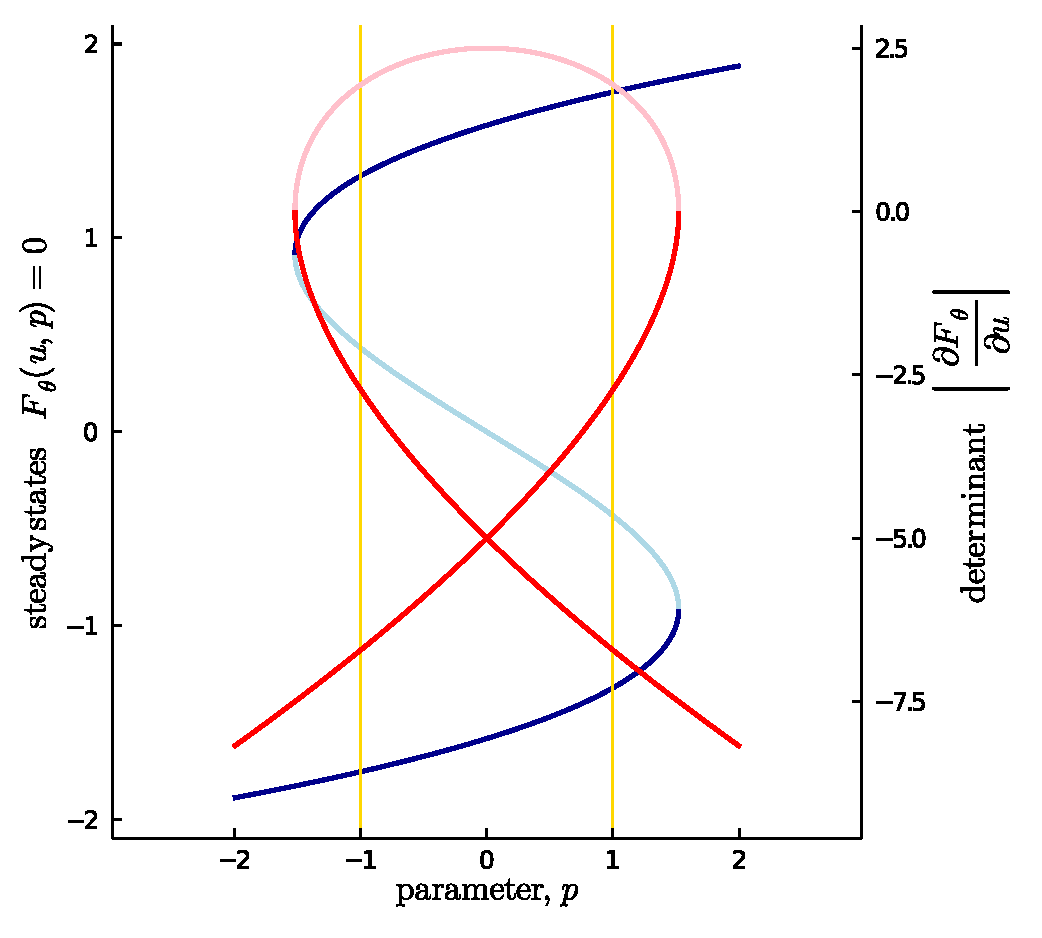
\includegraphics[width=11cm]{saddle-node}
\caption{Saddle-node model $\rates(z) = p + \theta_{1}u+\theta_{2}u^3$ with $\theta=(5/2,-1)$ and targets $\targets=\{-1,1\}$. Determinant in red. Lighter shades indicate the determinant crossing zero for unstable solutions}
\label{fig:saddle-node}
\end{figure}

\begin{figure}
\centering
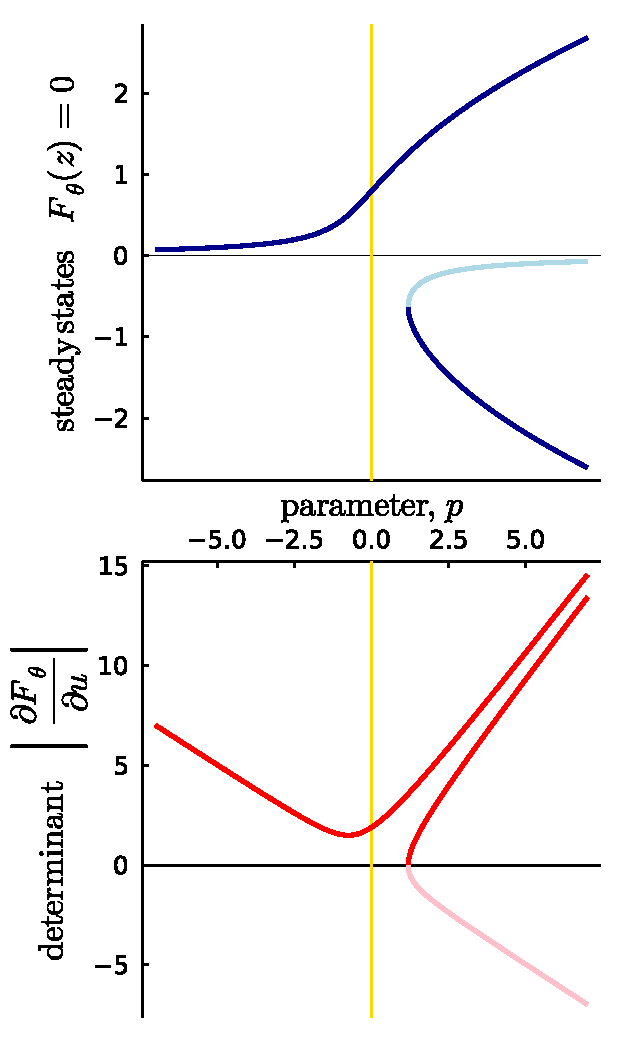
\includegraphics[width=11cm]{pitchfork}
\caption{Pitchfork model $\rates(z) = \theta_{1} + p u+\theta_{2}u^3$ with $\theta=(1/2,-1)$ and target $\targets=\{0\}$. Determinant in red. Lighter shades indicate the determinant crossing zero for unstable solutions}
\label{fig:pitchfork}
\end{figure}

\section{Proposed Method}
\subsection{Semi-supervised Cost Function}

\begin{figure}
    \centering
    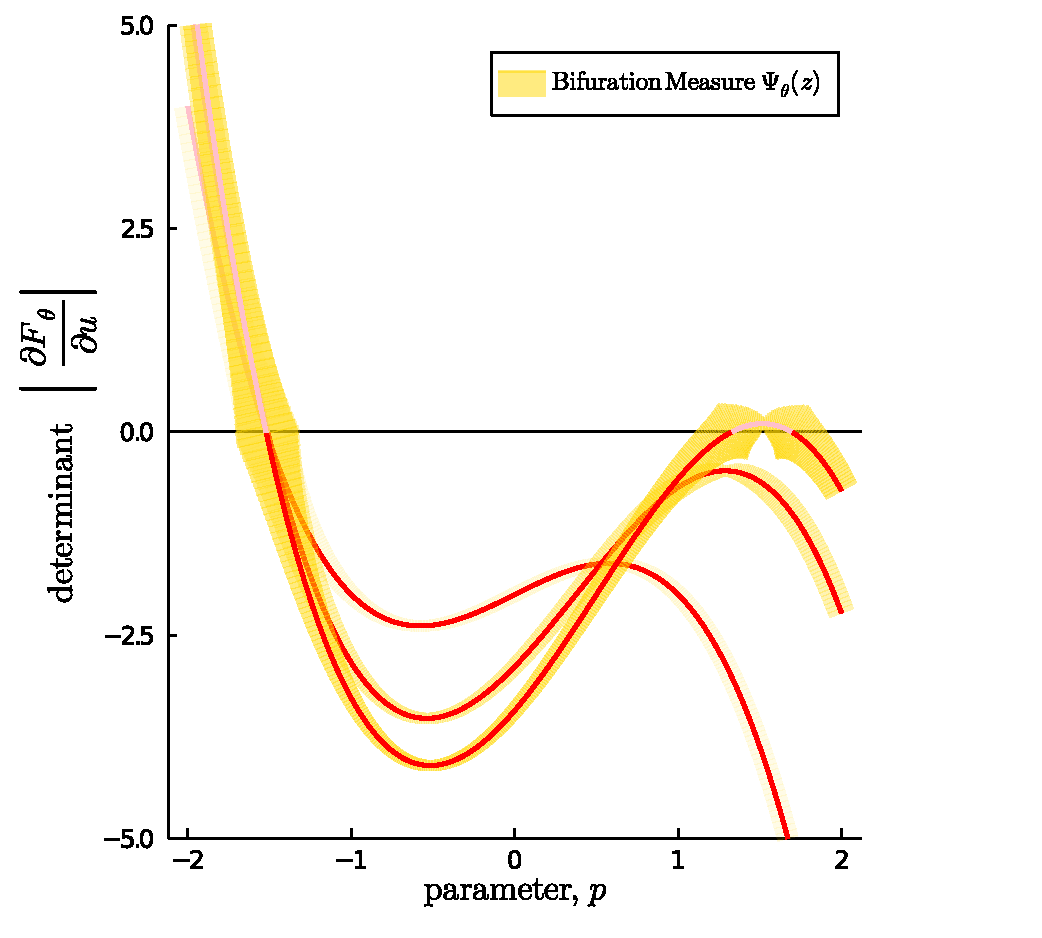
\includegraphics[width=7cm]{bifurcation-measure}
    \caption{Bifurcation measure $\measure(z)$ and determinant $\Det$ for two different bifurcation curves demonstrating how maximising the measure along the curve maintains the existing bifurcation marked by a circle, while encouraging new bifurcations marked by stars}
    \label{fig:bifurcation-measure}
\end{figure}

In order for predicted bifurcations $p(\theta)\in\predictions$ to match targets $p'\in\targets$ we need to evaluate an error term $|p(\theta)-p'|$. We expect this term to be some mean over the targets $\targets$ and predictions $\predictions(\theta)$. We choose a geometric mean over the predictions and an arithmetic mean over targets to account for cases where $|\predictions|\neq|\targets|$ and discourage multiple predictions matching the same target in cases where $|\predictions|\geq|\targets|$. This term only zero when each target is matched by at least one prediction
\begin{align}
    \frac{1}{|\targets|}\sum_{p'\in\targets}
    \prod_{p(\theta)\in\predictions}|p(\theta)-p'|
    ^{\frac{1}{|\predictions|}}
    \label{eq:supervised-term}
\end{align}
We can see from Figures \ref{fig:saddle-node} and \ref{fig:pitchfork} that predictions $p(\theta)$ can be identified by looking for points along the curve where the determinant $\Det=0$. Meanwhile the directional derivative along the bifurcation curve is finite $\frac{d}{ds}\Det\neq 0$ in the non-degenerate case. Using these quantities we can define a positive semi-definite measure $\measure(z)$ of zero crossings in the determinant along the bifurcation curve; as shown in Figure \ref{fig:bifurcation-measure} this can be used as a proxy for the probability of a bifurcation at location $p(\theta)$. The total bifurcation measure $\Psi(\theta)$ is written
\begin{align}
    \Psi(\theta):=\frac{
        \int_{\rates(z)=0}\!
        \measure(z)\,\mathrm{d}z
    }{
        \int_{\rates(z)=0}\!\
        \mathrm{d}z
    }
    \quad\mathrm{where}\quad
    \measure(z):=
    \left(1+\left|\frac{\Det}{\frac{d}{ds}\Det}\right|\right)^{-1}
    \label{eq:measure}
\end{align}
Here we denote $\int_{\rates(z)=0}\mathrm{d}z$ as the sum of the line integrals in $z\in\Reals^{N+1}$ defined by the steady states $\rates(z)=0$. The measure $\measure(z)=1$ at bifurcation points and goes to zero an odd number of times between bifurcations. This is because $\Det$ must eventually turn around in order to return back to zero, resulting in $\frac{d}{ds}\Det\rightarrow0$ and hence $\measure(z)\rightarrow0$ for each turning point. As $\Det$ diverges we approach regimes far away from any closest bifurcation and hence $\measure(z)\rightarrow0$. We would still like to have non-zero gradients with respect to $\theta$ in this regime, and therefore $\measure(z)$ was designed to go to zero slowly. The total measure $\Psi(\theta)$ is normalised such that $\Psi(\theta)\rightarrow1$ in the regimes where the observed parameter region $p$ is densely packed with bifurcations. The $\measure(z)$ is also invariant under certain classes of transformations on $\rates(z)$ which do not change bifurcation locations, proofs of which are provided in Appendix \ref{appendix:measure}. The measure is added to the supervised term as if it were a likelihood; this defines the semi-supervised cost function as
\begin{align}
    \loss(\theta|\targets):=
    \big(|\predictions|-|\targets|\big)\,\,\lambda \log\Psi(\theta)+
    \frac{1}{|\targets|}\sum_{p'\in\targets}
    \prod_{p(\theta)\in\predictions}|p(\theta)-p'|
    ^{\frac{1}{|\predictions|}}
    \label{eq:cost}
\end{align}
The pre-factor $|\targets|-|\predictions|$ in the unsupervised term ensures that the gradients are always pushing optimisers towards a state where $|\targets|=|\predictions|$. This can be seen as a step-wise annealing of the unsupervised term until the desired state is reached. Note that in principle while individual bifurcations $p(\theta)$ depend smoothly on $\theta$ the total number of predictions $|\predictions|$ does not. The gradient $\partial_{\theta}|\predictions|=0$ everywhere and is an infinite impulse at the exact locations where the number of predictions changes.

In practice optimisers are unlikely to hit those values of $\theta$ and we can safely drop the dependency. We may now proceed in taking gradients with respect to $\theta$ knowing that the only dependencies we need to track are for individual bifurcations $p(\theta)$ and total measure $\Psi(\theta)$
\begin{align}
    \frac{\partial\loss}{\partial\theta}=
    \big(|\predictions|-|\targets|\big)\,\lambda\,
    \frac{\partial \Psi}{\partial\theta}\Psi(\theta)^{-1}+
    \frac{1}{|\targets||\predictions|}\sum_{p'}
    \prod_{p(\theta)}|p(\theta)-p'|^{\frac{1}{|\predictions|}}
    \sum_{p(\theta)}\frac{\partial p}{\partial\theta}\left(p(\theta)-p'\right)^{-1}
    \label{eq:gradient}
\end{align}
In a similar vein to back-propagation through neural differential equations \cite{Chen2018NeuralEquations} we would like to be able to calculate the gradient $\frac{\partial\loss}{\partial\theta}$ without having to differentiate through the operations of the solver that finds the bifurcation curve $\rates(z)=0$ and the bifurcation locations $p(\theta)$. To calculate the gradient of the measure $\frac{\partial \Psi}{\partial\theta}$ we need to differentiate line integrals that depend on $\theta$. Fortunately this can be done by the application of the generalised Leibniz integral rule, details of which can be found in Appendix \ref{appendix:space-curve}.

The gradient of the bifurcation points $\frac{\partial p}{\partial\theta}$ is found by application of the implicit function theorem to a vector function $G_{\theta}:\Reals^{N+1}\rightarrow\Reals^{N+1}$ whos components represent the two constraints $\rates(z)=0$ and $\Det=0$. By following a similar strategy to that used by implicit layers \cite{Look2020DifferentiableLayers} we yield an $(N+1)\times M$ Jacobian representing a deformation field \cite{Jos2011OnSurface} for each $\theta$ direction. The gradient we are looking for becomes
\begin{align}
    \frac{\partial p}{\partial\theta} = -\hat{p}\cdot\left.\frac{\partial G_{\theta}}{\partial z}^{-1}
    \frac{\partial  G_{\theta}}{\partial\theta}\right|_{G_{\theta}(z)=0}
    \quad\mathrm{where}\quad
    G_{\theta}(z):=\begin{bmatrix}\rates(z)\\\Det\end{bmatrix}
\end{align}
Here $\hat{p}$ is a unit vector in $z\in\Reals^{N+1}$ that picks out the deformations along the $p$-direction. We can see this calculation involves inverting an $(N+1)\times(N+1)$ Jacobian $\frac{\partial G_{\theta}}{\partial z}$. The determinant of this Jacobian goes to zero when $\frac{d}{ds}\Det=0$. This further justifies our choice for measure $\measure(z)$ which discourages such cases.

The cost function is piece-wise smooth and differentiable with undefined gradients only in parameter regions where the number of predictions $|\predictions|$ changes. Given a set of solutions to $\rates(z)=0$ and locations $p(\theta)$ which additionally satisfy $\Det=0$, the gradient $\frac{\partial\loss}{\partial\theta}$ can evaluated using automatic differentiation methods.

\subsection{Implementation}
\label{section:implementation}
%/ move to appendix?
Here provide a high-level view of Algorithm \ref{alg:optimisation-loop}. We use \texttt{BifurcationKit.jl} \cite{Veltz2019PseudoArcLengthContinuation.jl} to calculate bifurcation diagrams, which requires the rate function $\rates$, its Jacobian $J_\theta$ which can be calculated using \texttt{ForwardDiff.jl} \cite{Revels2016Forward-ModeJulia}, and an initial guess $u_0$ at an initial parameter $p_0$. Let this algorithm be called by function \texttt{getSteadyStates} and return the steady states that form the integration region $\steadystates$ and a new guess $u_0$ that is the true steady state at $p_0$.

The algorithm also takes hyperparameters $\beta$ which will contain arclength step sizes, eigenvalue and Newton solver options and unsupervised correction factor $\lambda$. The adaptive hyperparameter update is done by \texttt{updateHyperparameters} and should depend on the current solutions $\steadystates$ and the targets $\targets$. The step sizes and solver options should adapt to the expected space of the solutions $\steadystates$ so that the waiting time between iterations is minimised. The unsupervised correction factor $\lambda$ should be large when there are no predicted bifurcations and decrease as the number of predicted bifurcations approaches the number of targets.

The evaluation of the cost gradient is done by \texttt{costGradient} using \texttt{ForwardDiff.jl} \cite{Revels2016Forward-ModeJulia} which has a large repository of chain rules that it uses to correctly evaluate derivatives. At the time of writing this paper the repository does not include the Leibniz rule \cite{Flanders1973DifferentiationSign} for implicitly defined line integrals, and we therefore define additional rules that implement the results shown in Appendix \ref{appendix:space-curve} and \ref{appendix:deformation}. The cost gradient is used by \texttt{updateParameters}, which can be any gradient-based optimiser such as ADAM or Momentum gradient decent, to update the parameters $\theta$.

In practice the bifurcation curve is only evaluated in a finite region $p\in\Omega$ which includes the targets $\targets$. We are now ready to write down the semi-supervised cost function for a bifurcation curve defined by $\rates(z)=0$ in an observed region $p\in\Omega$.

\begin{algorithm*}[H]
\label{alg:optimisation-loop}
\SetAlgoLined
\textbf{Inputs} Function $F_{\theta}:\mathbb{R}^{N+1}\rightarrow\mathbb{R}^{N}$ for $u\in\mathbb{R}^N$ and $p\in\mathbb{R}$\\ target bifurcations $\mathcal{D}=\{p_1\dots p_K:p\in\Omega\}$ and convergence tolerance $\varepsilon$\\
\textbf{Output} Optimised $\theta\in\mathbb{R}^M$ that satisfy targets $\targets$\\
$u_0\leftarrow\mathrm{rand}\in\mathbb{R}^{N}$\quad\,$\theta\leftarrow\mathrm{rand}\in\mathbb{R}^{M}$\\
$\beta\leftarrow\texttt{getHyperparameters}(\targets)$\\
\While{$\mathrm{tolerance}(\beta)>\varepsilon$}{
  $\steadystates,u_0\leftarrow\texttt{getSteadyStates}(F_{\theta},u_0,\beta)$\\
  $\beta\leftarrow\texttt{updateHyperparameters}(\beta,\steadystates,\targets)$\\
  $\partial L\leftarrow\texttt{costGradient}(F_{\theta},\steadystates,\targets,\beta)$\\
  $\theta\leftarrow\texttt{updateParameters}(\theta,\partial L,\beta)$
}
\caption{Bifurcation Optimisation Loop}
\end{algorithm*}

\section{Experiments \& Results}

\subsection{Minimal Models}
Figures \ref{fig:saddle-node:results} and \ref{fig:pitchfork:results} show example optimisations of $(\theta_1,\theta_2)$ for the minimal saddle-node and pitchfork models respectively. The magnitude of the correction factor $\lambda=0$ when bifurcations are present and $\lambda\neq0$ otherwise. Optimisation trajectories approach lines of global minima in the cost function, which represent a set of geometrically equivalent models, depicted in the right panels. Two bifurcation curves are geometrically equivalent if the number, type and locations of bifurcations match.

We can see that the geometrically equivalent lines are contained within larger basins defined by $\lambda=0$ where the correct number and type of bifurcations are present $p\in\Omega$, but do not match the locations of targets $\targets$. All models within this basin are in some sense topologically equivalent. This hierarchical classification allows us to identify the set of models that satisfy observed qualitative behaviour \cite{Stumpf2019ParameterBifurcations} before any attempt at inferring kinetic parameters, which is done by choosing a model along the line of geometrically equivalent models.

Optimisation trajectories for the two minimal models appear mostly circumferential. This is because the models were set up such that the radial direction from the origin in $\theta$ space mostly scale kinetics whereas the circumferential direction changes the bifurcation topology. This suggests that the gradients of our cost function seek to change model geometry over kinetics.

\begin{figure}
\centering
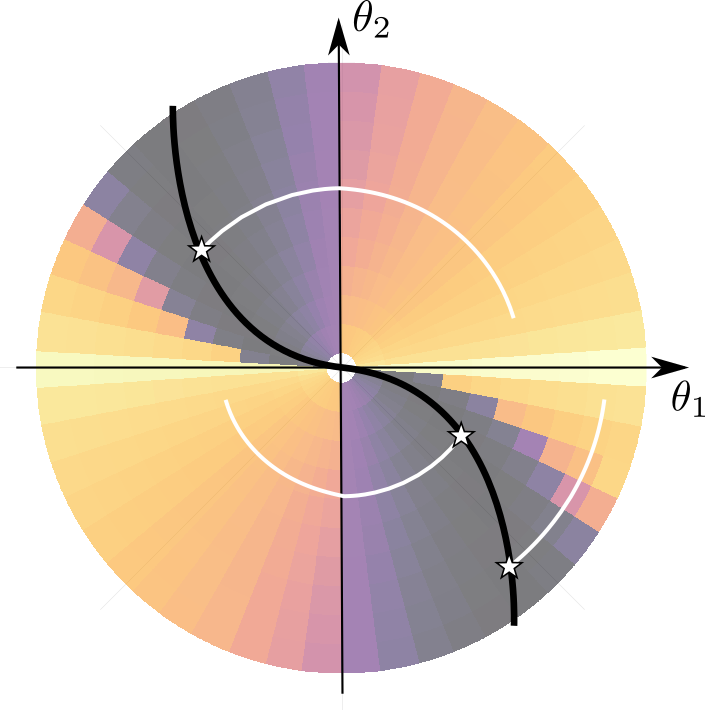
\includegraphics[width=6cm]{saddle-landscape.png}
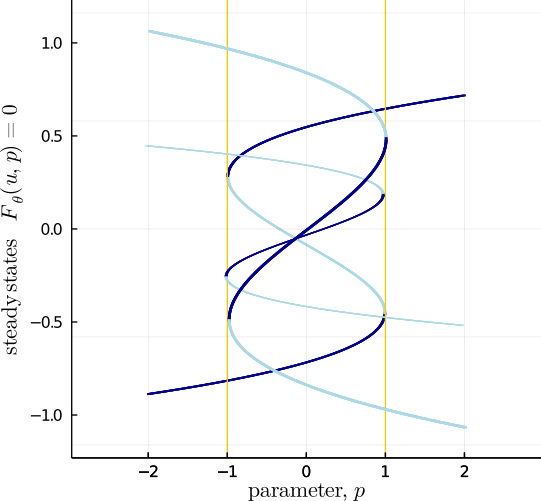
\includegraphics[width=6cm]{saddle-optima.png}
\caption{Saddle-node model $\rates(u,p) = p + \theta_{1}u+\theta_{2}u^3$ optimised with respect to targets $\targets=\{-1,1\}$ in observation region $\Omega\in[-2,2]$. The right panel shows bifurcations diagrams for the three optima marked by stars on the left panel. The optimisation trajectories in white follow the gradient of the cost, approaching the black line of global minima in the left panel}
\label{fig:saddle-node:results}
\end{figure}

\begin{figure}
\centering
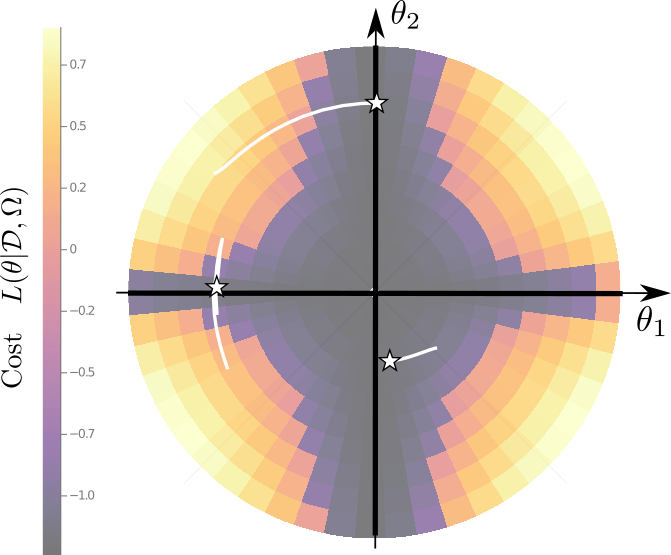
\includegraphics[width=6cm]{pitchfork-landscape.png}
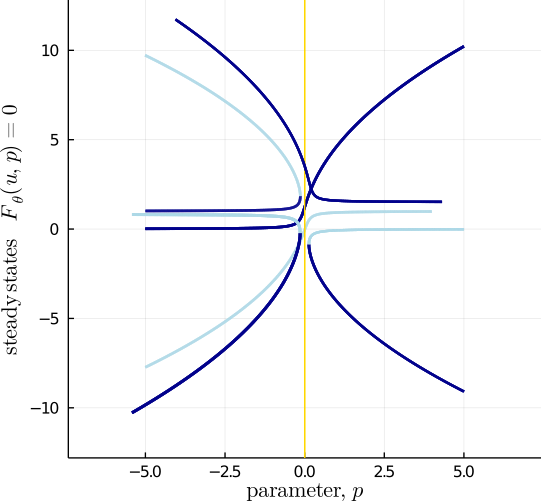
\includegraphics[width=6cm]{pitchfork-optima.png}
\caption{Pitchfork model $\rates(u,p) = \theta_{1} + u p +\theta_{2}u^3$ optimised with respect to targets $\targets=\{0\}$ in observation region $\Omega\in[-5,5]$. The right panel shows bifurcations diagrams for the three optima marked by stars on the left panel. The optimisation trajectories in white follow the gradient of the cost, approaching the black lines of global minima in the left panel}
\label{fig:pitchfork:results}
\end{figure}

\subsection{Genetic Toggle Switch | \textit{in progress}}
In this section we optimise a model where the states share a Hill function relationship; these models often emerge from mass action kinetics and are used to model species concentrations. By not restricting the sign of the coefficients $a_1,a_2$ we can recover both activator and inhibitor relationships.
\begin{equation}
    \partial_t u_1 = \frac{\varepsilon_1 + a_1 u_2^2} { k_1^2 + u_2^2 } - \mu_1 u_1 \quad
    \partial_t u_2 = \frac{p + a_2 u_1^2} { k_2^2 + u_1^2 } - \mu_2 u_2
    \label{eq:two-state}
\end{equation}
Figure \ref{fig:two-state-optima} shows a UMAP embedding of the optimal parameter basins, represented as point clouds. 16 distinct clusters are obtained using DBSCAN. Each cluster corresponds to a kinetically different model regions that are qualitatively equivalent. See Appendix \ref{appendix:clusters} for models that represent the centroid of each cluster.
 
\begin{figure}
\centering
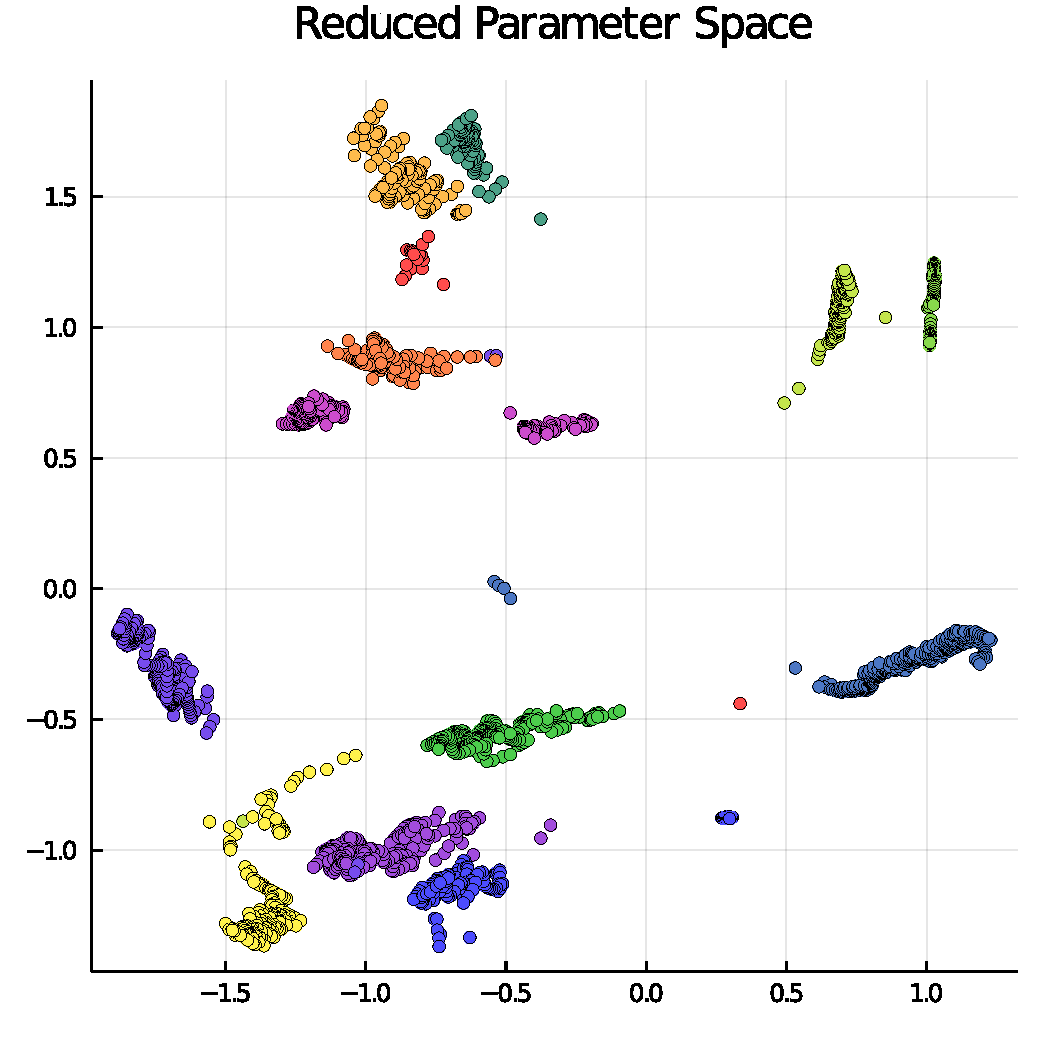
\includegraphics[width=11cm]{two-state-optima}
\caption{Reduced dimensionality plot of optimal $\theta^*$ for the two state model \eqref{eq:two-state} for $\targets=\{4,5\}$}
\label{fig:two-state-optima}
\end{figure}
 
\section{Conclusion \& Broader Impact | \textit{in progress}}
\begin{itemize}
    \item Taking steps towards an efficient and single method for searching and matching bifurcations
    \item A demonstrating of the powerful combination of differential geometry and implicit layers
    \item Future directions include extending this routine for Hopf bifurcations and PDEs
    \item Computational limitations
\end{itemize}

% \section*{Checklist}
% \begin{enumerate}

\item For all authors...
\begin{enumerate}
  \item Do the main claims made in the abstract and introduction accurately reflect the paper's contributions and scope?
    \answerYes{}
  \item Did you describe the limitations of your work?
    \answerYes{Implementation only covers co-dimension one bifurcations. Does not scale well for PDEs. See discussion in Section \ref{}}
  \item Did you discuss any potential negative societal impacts of your work?
    \answerNA{}
  \item Have you read the ethics review guidelines and ensured that your paper conforms to them?
    \answerYes{}
\end{enumerate}

\item If you are including theoretical results...
\begin{enumerate}
  \item Did you state the full set of assumptions of all theoretical results?
    \answerNA{This paper applies existing theorems. See Section \ref{section:method}}
	\item Did you include complete proofs of all theoretical results?
    \answerNA{We include derivations to guide the reader in Appendices}
\end{enumerate}

\item If you ran experiments...
\begin{enumerate}
  \item Did you include the code, data, and instructions needed to reproduce the main experimental results (either in the supplemental material or as a URL)?
    \answerYes{All figures are unit tests in the GitHub repository for \texttt{BifurcationFit.jl}}
  \item Did you specify all the training details (e.g., data splits, hyperparameters, how they were chosen)?
    \answerYes{ADAM was used with various hyper-parameters}
	\item Did you report error bars (e.g., with respect to the random seed after running experiments multiple times)?
    \answerYes{See Figure \ref{fig:scaling} and }
	\item Did you include the total amount of compute and the type of resources used (e.g., type of GPUs, internal cluster, or cloud provider)?
    \answerYes{See Figure \ref{fig:scaling}}
\end{enumerate}

\item If you are using existing assets (e.g., code, data, models) or curating/releasing new assets...
\begin{enumerate}
  \item If your work uses existing assets, did you cite the creators?
    \answerYes{\cite{Veltz2019PseudoArcLengthContinuation.jl,Revels2016Forward-ModeJulia,Flux}}
  \item Did you mention the license of the assets?
    \answerNo{All assets have been release under MIT}
  \item Did you include any new assets either in the supplemental material or as a URL?
    \answerYes{All code available under \texttt{github.com/gszep/BifurcationFit.jl} }
  \item Did you discuss whether and how consent was obtained from people whose data you're using/curating?
    \answerNA{}
  \item Did you discuss whether the data you are using/curating contains personally identifiable information or offensive content?
    \answerNA{}
\end{enumerate}

\item If you used crowdsourcing or conducted research with human subjects...
\begin{enumerate}
  \item Did you include the full text of instructions given to participants and screenshots, if applicable?
    \answerNA{}
  \item Did you describe any potential participant risks, with links to Institutional Review Board (IRB) approvals, if applicable?
    \answerNA{}
  \item Did you include the estimated hourly wage paid to participants and the total amount spent on participant compensation?
    \answerNA{}
\end{enumerate}

\end{enumerate}

\bibliography{refs}
\bibliographystyle{ieeetr}

\section*{Appendix}
\appendix
\section{Supplementary Figures}

\begin{figure}[H]
\centering
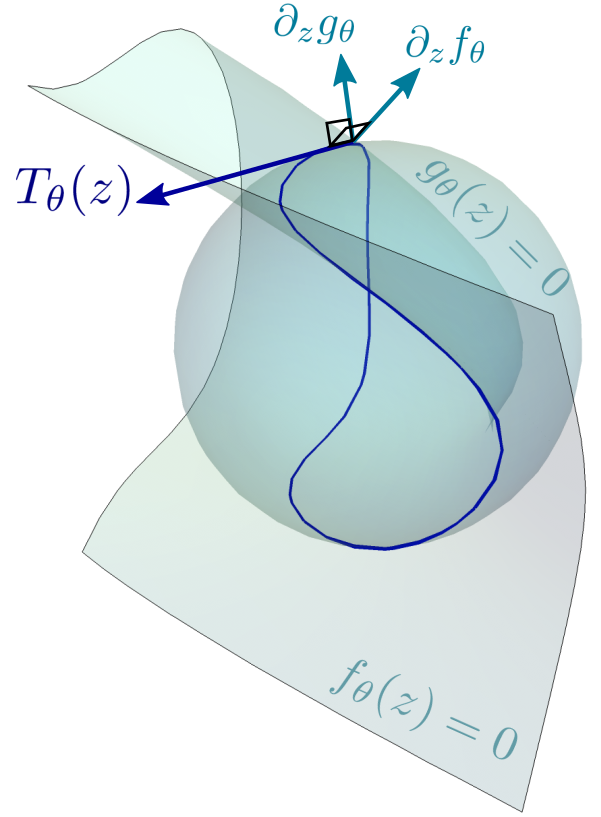
\includegraphics[width=5cm]{implicit-surfaces}
\caption{Two implicit surfaces $f_{\theta}(z)=0$ and $g_{\theta}(z)=0$ in $\mathbb{R}^3$ intersecting to form a space curve which is tangent to field $\tangent(z)$ and perpendicular to gradients $\partial_{z}f_{\theta}$ and $\partial_{z}g_{\theta}$}
\label{fig:implicit-surfaces}
\end{figure}

\section{Gradient of Space Curve}
\label{appendix:space-curve}

Suppose there exists a one dimensional space curve $\mathcal{C(\theta)}$ embedded in $z\in\Reals^{N+1}$ whos geometry changes depending on input parameters $\theta\in\Reals^M$. This curve could be open or closed and changes in $\theta$ could change the curve topology as well. Let the function $\gamma_{\theta}:\Reals\rightarrow\Reals^{N+1}$ be a parameterisation of the position vector along the curve within a fixed domain $s\in\mathcal{S}$. Note that the choice of parameterisation is arbitrary and our results should not depend on this choice. Furthermore, if we parametrise the curve $\mathcal{C}(\theta)$ with respect to a fixed domain $\mathcal{S}$ the dependence on $\theta$ is picked up by the parameterisation $\gamma_{\theta}(s)$. We can write a line integral of any scalar function $L_{\theta}:\Reals^{N+1}\rightarrow\Reals$ on the curve as
\begin{align}
    L(\theta):=
    \int_\mathcal{C(\theta)}\! L_{\theta}(z)\,\mathrm{d}z
    =\int_\mathcal{S}\! L_{\theta}(z)\left|\frac{d\gamma_{\theta}}{ds}\right|\mathrm{d}s_{\,\,z=\gamma_{\theta}(s)}
\end{align}
where $\left|\frac{d\gamma_{\theta}}{ds}\right|$ is the magnitude of tangent vectors to the space curve and we remind ourselves that the integrand is evaluated at $z=\gamma_{\theta}(s)$. We would like to track how this integral changes with respect to $\theta$. The total derivative with respect to $\theta$ can be propagated into the integrand \cite{Flanders1973DifferentiationSign} as long as we keep track of implicit dependencies
\begin{align}
    \frac{dL}{d\theta} &=\int_\mathcal{S}
    \left|\frac{d\gamma_{\theta}}{ds}\right|
    \left(
        \frac{\partial L}{\partial\theta}+
        \frac{\partial L}{\partial z}\cdot
        \frac{dz}{d\theta}
    \right)
    +L_{\theta}(z)\frac{d}{d\theta}\left|\frac{d\gamma_{\theta}}{ds}\right|
    \mathrm{d}s_{\,\,z=\gamma_{\theta}(s)}
    % \\&=\int_\mathcal{C(\theta)}
    %     \frac{\partial L}{\partial\theta}+
    %     \frac{\partial L}{\partial z}\cdot
    %     \frac{dz}{d\theta}
    % +L_{\theta}(z)\frac{d}{d\theta}\log\left|\frac{d\gamma_{\theta}}{ds}\right|
    % \mathrm{d}z
\end{align}
Here we applied the total derivative rule in the first term due to the implicit dependence of $z$ on $\theta$ through $z=\gamma_{\theta}(s)$. Applying the chain rule to the second term
\begin{align}
    \frac{d}{d\theta}\left|\frac{d\gamma_{\theta}}{ds}\right|=
    \left|\frac{d\gamma_{\theta}}{ds}\right|^{-1}
    \frac{d\gamma_{\theta}}{ds}\cdot\frac{d}{d\theta}
    \left(\frac{d\gamma_{\theta}}{ds}\right)
\end{align}
By choosing an $s$ that has no implicit $\theta$ dependence we can commute derivatives
\begin{align}
    \frac{d}{d\theta}\left(\frac{d\gamma_{\theta}}{ds}\right)
    = \frac{d}{ds}\left(\frac{d\gamma_{\theta}}{d\theta}\right)
    \quad\Rightarrow\quad
    \frac{d}{d\theta}\left|\frac{d\gamma_{\theta}}{ds}\right|=
    \left|\frac{d\gamma_{\theta}}{ds}\right|^{-1}
    \frac{d\gamma_{\theta}}{ds}\cdot\frac{d}{d s}
    \left(\frac{d\gamma_{\theta}}{d\theta}\right)
\end{align}
To proceed we note that the unit tangent vector can be written as an evaluation of a tangent field $\hat{T}_{\theta}(z)$ defined in the whole domain $z\in\Reals^{N+1}$ along the parametric curve $z=\gamma_{\theta}(s)$. The unit tangent field may disagree with the tangent given by $\frac{d\gamma_{\theta}}{ds}$ up to a sign
\begin{align}
    \left.\hat{\tangent}(z)\right|_{z=\gamma_{\theta}(s)}=
    \pm\left|\frac{d\gamma_{\theta}}{ds}\right|^{-1}\frac{d\gamma_{\theta}}{d s}
\end{align}
this leads to numerically verified result%\todo{perhaps not valid in general?}
\begin{align}
    \frac{d}{d\theta}\left|\frac{d\gamma_{\theta}}{ds}\right|=
    \left|\frac{d\gamma_{\theta}}{ds}\right|\left(
   \hat{\tangent}(z)\cdot\frac{\partial }{\partial z}\left(\frac{d\Gamma_{\theta}}{d \theta}\right)\cdot
   \hat{\tangent}(z)
    \right)_{z=\gamma_\theta(s)}
    \label{eq:divergence-term}
\end{align}

\section{Deformation of Implicit Surfaces}
\label{appendix:deformation}
It is possible to find the normal deformation of the implicit space curves due to changes in $\theta$. This can be done by taking the total derivative of the implicit equation defining the level set
\begin{align}
    \frac{d\rates(z)}{d\theta}=\frac{\partial F}{\partial\theta}+
    \frac{\partial F}{\partial z}\cdot\frac{d z}{d \theta}
\end{align}

We can rearrange for $\frac{d z}{d \theta}$ using the Moore-Penrose inverse of the rectangular Jacobian matrix $\frac{\partial F}{\partial z}$ which appeared in equation \eqref{eq:tangent-field}. Since the level set is defined by $\rates(z)=0$ the total derivative along the level set $d\rates(z)=0$ and we arrive at an expression for the deformation field \cite{Jos2011OnSurface}
\begin{align}
    \frac{d z}{d \theta} = - \frac{\partial F}{\partial z}^\top
    \left(\,
        \frac{\partial F}{\partial z}\,\frac{\partial F}{\partial z}^\top
    \right)^{-1}
    \frac{\partial F}{\partial\theta}
\end{align}
The tangential component of the deformation field is not uniquely determined because there is no unique way of parameterising a surface. This is the subject of many computer graphics papers \cite{Jos2011OnSurface,Tao2016Near-IsometricTracking,Fujisawa2013CalculationInvariance}. We are however not interested in the continuous propagation of a mesh - as is the subject of those papers. In fact we are looking for a deformation field that is orthogonal to the tangent vector $\hat{\tangent}(z) \cdot\frac{d z}{d\theta} =0$ for the space curve, and therefore letting the tangential component of the deformation equal zero is a valid choice and we can it instead of the parameterised deformation
% \todo{this is possibly quite shifty. Is this really valid?}
\begin{align}
    \frac{d \gamma_{\theta}}{d\theta} \rightarrow \frac{d z}{d\theta}
\end{align}
To summarise we now have the gradient of our line integral only in terms of the implicit function defining the integration region.
\begin{align}
    \frac{d L}{d\theta} =\int_{\rates(z)=0}
        \frac{\partial L}{\partial\theta}+
        \frac{\partial L}{\partial z}\cdot
        \varphi_{\theta}(z)
    +L_{\theta}(z)\,\,
    \hat{\tangent}(z)\cdot\frac{\partial \varphi}{\partial z}\cdot\hat{\tangent}(z)
    \,\mathrm{d}z\qquad\qquad\\
    \mathrm{where}\quad
    \hat{\tangent}(z):= \frac{\tangent(z)}{|\tangent(z)|}
    \qquad
    \tangent(z):=
    \left|\begin{matrix}
        \hat{z} \\
        \,\partial_{z}\rates\,
    \end{matrix}\right|
    \qquad
    \varphi_{\theta}(z) :=
- \frac{\partial F}{\partial z}^\top
    \left(\,
        \frac{\partial F}{\partial z}\,\frac{\partial F}{\partial z}^\top
    \right)^{-1}
    \frac{\partial F}{\partial\theta}
\end{align}
We have settled on choosing normal deformations which we will call $\varphi_\theta(z)$. The above result can be seen a the generalised Leibniz rule \cite{Flanders1973DifferentiationSign} for the case of line integration regions. The last integrand term can be seen as the divergence the vector field $\varphi_\theta(z)$ projected onto the one dimensional space curve.


\subsection{Bifurcation Curves as Tangent Fields}
\label{appendix:tangent-fields}

Let each component of the vector function $\rates$ in the model \eqref{eq:model} implicitly define a surface embedded in $\Reals^{N+1}$. Let's assume that the intersection of these $N$ surfaces exists and is not null or degenerate, then the steady states of \eqref{eq:model} must be a set of one dimensional space curves in $z\in\Reals^{N+1}$ defined by
\begin{align}
    \rates(z) = 0
\end{align}
An expression for the field $\tangent(z)$ tangent to the set of curves would allow us to take derivatives and integrals along the bifurcation curve. This is exactly what we need to do to evaluate our cost function \ref{eq:cost}. Fortunately the tangent field can be constructed by ensuring it is perpendicular to the gradient $\partial_z$ of each component of $\rates$ as illustrated by an example two component system in Figure \ref{fig:implicit-surfaces}. The tangent field $\tangent(z)$ can be constructed perpendicular to all gradient vectors using the properties of the determinant \cite{Goldman2005CurvatureSurfaces}
\begin{align}
    \tangent(z):=
    \label{eq:tangent-field}
    \left|\begin{matrix}
        \hat{z} \\
        \,\partial_{z}\rates\,
    \end{matrix}\right|
    \qquad\tangent : \Reals^{N+1}\rightarrow\Reals^{N+1}\\
    =\sum_{i=1}^{N+1}\hat{z}_{i}(-1)^{i+1} \left|\frac{\partial \rates}{\partial(z\setminus z_{i}) }\right|
\end{align}
where $\hat{z}$ is a collection of unit basis vectors in the $\Reals^{N+1}$ space and $\partial_{z}\rates$ is an $N\times(N+1)$ rectangular Jacobian matrix of partial derivatives and $z\setminus z_{i}$ denotes the $N$ dimensional vector $z$ with component $z_{i}$ removed. This construction ensures perpendicularity to any gradients of $\rates$
\begin{align}
    \tangent(z)\cdot\partial_z f_{\theta} =
    \left|\begin{matrix}
        \partial_z f_{\theta} \\
        \,\partial_{z}\rates\,
    \end{matrix}\right|
    \quad =0 \quad\forall f_{\theta}\in \rates
\end{align}
since the determinant of any matrix with two identical rows or columns is zero. Note that the tangent field $\tangent(z)$ is actually defined for all values of $z$ where adjacent field lines trace out other level sets where $\rates(z)\neq0$. Furthermore deformations with respect to $\theta$ are always orthogonal to the tangent
\begin{align} % \todo{numerically true. analytic proof?}
    \tangent(z)\cdot\frac{d\tangent}{d\theta}=0
\end{align}
\begin{figure}
\centering
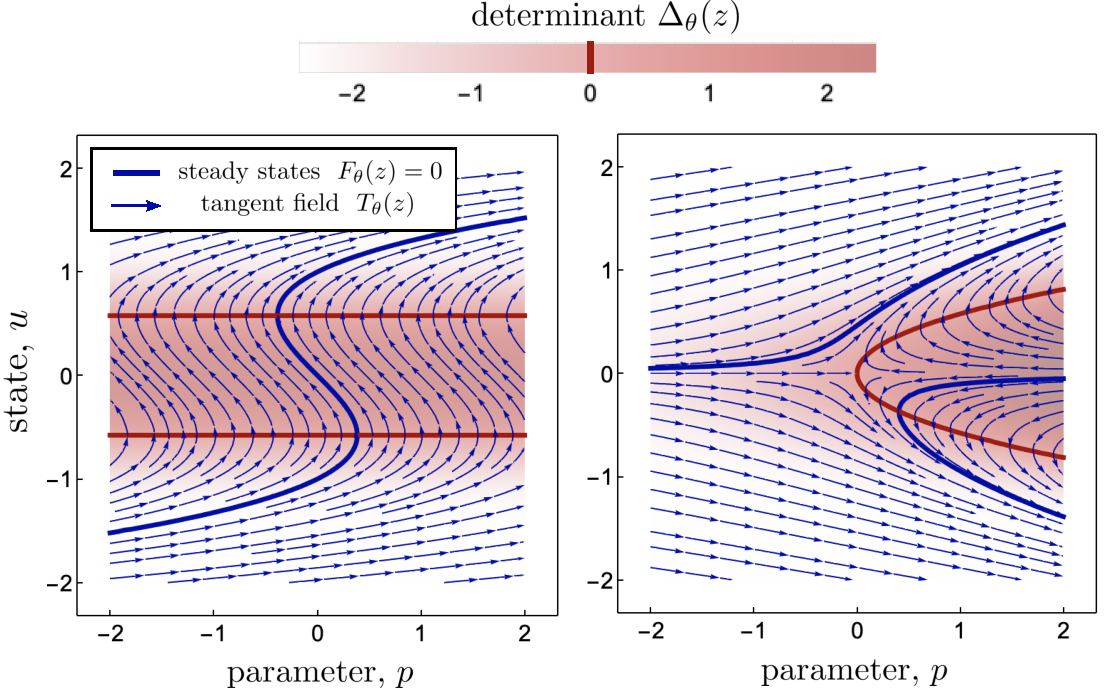
\includegraphics[width=13cm]{determinant-field}
\caption{Left/Right : Determinant $\Det$ and tangent field $\tangent(z)$ for the saddle-node/pitchfork models for some set values of $\theta$ revealing that $\Det=0$ defines bifurcations}
\label{fig:determinant-field}
\end{figure}
Figure \ref{fig:determinant-field} shows how the bifurcation curve defined by $\rates(z)=0$ picks out one of many level sets or traces in tangent field $\tangent(z)$ for the saddle and pitchfork. The tangent field $\tangent(z)$ can always be analytically evaluated by taking the determinant in \eqref{eq:tangent-field}. We will proceed with calculations on $\tangent(z)$ in the whole space $z$ and pick out a single trace by solving $\rates(z)=0$ later. For our two models
\begin{align}
    \underset{\mathrm{saddle-node\,\,model}}{
    \tangent(z)=\hat{u}-(\,3\theta_2 u^2+\theta_1\,)\,\hat{p}}
    \qquad\qquad
    \underset{\mathrm{pitchfork\,\,model}}{
    \tangent(z)=u\hat{u}-(\,3\theta_2 u^2+p\,)\,\hat{p}}
    \label{eq:tangent-field-examples}
\end{align}
Figure \ref{fig:determinant-field} reveals that $\Det=0$ is also a level set and that the intersection with level set $\rates(z)=0$ defines the bifurcations at specific parameter $\theta$. In this particular setting we can see that the tangent field $\tangent(z)$ only folds when $\Det=0$. Plotting the value of the determinant along $\rates(z)=0$ from Figure \ref{fig:determinant-field} would give rise to Figures \ref{fig:minimal-models}. The directional derivative of the determinant $\Det$ along the tangent field $\tangent(z)$ is defined as
\begin{align}
    \frac{d}{ds}\Det := \hat{\tangent}(z) \cdot \frac{\partial}{\partial z}\Det 
\end{align}
where $\hat{\tangent}(z)$ is the unit tangent field. 


\section{Bifurcation Measure}
\label{appendix:measure}


\section{Simplification of two-state model}

Consider the general two-state model:
\begin{equation}
    \dfrac{dv_i}{dt} = \dfrac{a_i + b_i (K_i v_j)^2}{1 + (K_i v_j)^2} - \mu_i v_i
\end{equation}

Without loss of generality, we can rescale $v_i = U_i u_i$. Then,
\begin{equation}
    \dfrac{U_idu_i}{dt} = \dfrac{a_i + b_i (K_i U_j u_j)^2}{1 + (K_i U_j u_j)^2} - \mu_i U_i u_i
\end{equation}

Dividing through by $U_i$, we obtain
\begin{equation}
    \dfrac{du_i}{dt} = \dfrac{\frac{a_i}{U_i} + \frac{b_i}{U_i} (K_i U_j u_j)^2}{1 + (K_i U_j u_j)^2} - \mu_i u_i
\end{equation}

By choosing $U_i = b_i$, the model reduces to:
\begin{equation}
    \dfrac{du_1}{dt} = \dfrac{\hat{a}_1 + (p u_2)^2}{1 + (p u_2)^2} - \mu_1 u_1, \quad
    \dfrac{du_2}{dt} = \dfrac{\hat{a}_2 + (k u_1)^2}{1 + (k u_1)^2} - \mu_2 u_2
\end{equation}
where $p = \frac{K_1}{\sqrt{b_1}}$ and $k = \frac{K_2}{\sqrt{b_2}}$.

\end{document}
